%%%%%%%%%%%%%%%%%%%%%%%%%%%%%%%%%%%%%%%%%%%%%%%%%%%%%%%%%%%%%%%%%
%  _____       ______   ____									%
% |_   _|     |  ____|/ ____|  Institute of Embedded Systems	%
%   | |  _ __ | |__  | (___    Wireless Group					%
%   | | | '_ \|  __|  \___ \   Zuercher Hochschule Winterthur	%
%  _| |_| | | | |____ ____) |  (University of Applied Sciences)	%
% |_____|_| |_|______|_____/   8401 Winterthur, Switzerland		%
%																%
%%%%%%%%%%%%%%%%%%%%%%%%%%%%%%%%%%%%%%%%%%%%%%%%%%%%%%%%%%%%%%%%%

\chapter{MIDI-Steuerung}\label{chap.midi}

\section{Das MIDI-Kommunikationsprotokoll}\label{sect.midi_spezification}

Werden MIDI Daten übermittelt, so unterscheidet der Standard zwei Typen an Daten \citep{Midi_specification}.

\subsection{MIDI-Daten-Typen}\label{datentypen}

\subsubsection*{Status Bytes}

Status Bytes sind 8 Bit lang und das MSB ist immer logisch \lstinline|'1'|. Status Bytes dienen dem Identifizieren der nachfolgenden Data Bytes. Das Status Byte definiert die Datenstruktur der folgenden Data Bytes.

MIDI behält einen Status, bis ein neues Status Byte folgt. Dieses Verhalten ist als Running Status bezeichnet. Dieses Verhalten ist für Polyphonie relevant, da der Zustand bleibt, bis ein neues Status Byte folgt.

\subsubsection*{Data Bytes}

Gemäss Spezifikation folgen einem Status Byte ein oder zwei Bytes. Das MSB ist immer logisch \lstinline|'0'|. Die Werte können von \lstinline|0x00| bis \lstinline|0x7F| sein. Das bedeutet, dass MIDI maximal 128 Noten unterscheiden kann.

Data Bytes können unterschiedliche Informationen enthalten. Im Kontroller sind Notenwerte, Geschwindigkeit des Anschalges relevant.

Je nach dem Status Byte werden die Data Byte anders interpretiert. 

\begin{quote}
``Empfänger sollen so konzipiert sein, dass zuerst alle Data Bytes empfangen werden und ein neues Status Byte kommt. Danach werden ungültige Daten verworfen. Einzige Ausnahme ist der Running Status, bei dem nicht bis zum Ende gewartet wird.'' \citep{Midi_specification}.
\end{quote}

\subsubsection*{Ungültige Bytes}

\begin{quote}
``Alle Status Bytes, die nicht implementierte Funktionen enthalten und alle ihnen folgenden Data Bytes sollen vom Empfänger verworfen werden.'' \citep{Midi_specification}
\end{quote}

MIDI Geräte sollen ausdrücklich beim Ein- und Abstellen darauf bedacht sein, dass keine undefinierten Bytes gesendet werden \citep{Midi_specification}.\\
Diese Anforderung ist wichtig beim Implementieren der Finite State Machine und der Test Bench (siehe Kapitel \ref{chap.testen})

\subsubsection*{Midi Bytes binär}\label{midi_binaer}

\begin{itemize}
	\item \lstinline|"0xxx xxxx"|: Definition Data Byte
	\item \lstinline|"1xxx xxxx"|: Definition Status Byte
	\item \lstinline|"1000 xxxx"|: Definition NOTE OFF
	\item \lstinline|"1001 xxxx"|: Definition NOTE ON
	\item \lstinline|"1010 xxxx"|: Definition POLYPHONY
	\item \lstinline|"100x xxxx"|: Erste drei Bits der Status Bytes NOTE ON (0x90) und NOTE OFF (0x80)
\end{itemize}

\subsection{Zwei MIDI-Noten-Modi}\label{note_modes}

\subsubsection{Datenstruktur}

Die Datenstruktur der zwei MIDI-Noten-Modi beginnt mit dem Status Byte (grau in der Abbildung \ref{fig.testbench_single_Mode}). Es folgt der Notenwert (hier Dummy-Wert von 0x11 eingetragen) und die Geschwindigkeit. Letztere hat im Single Mode keine spezifische Bedeutung, im Polyphony Mode bestimmt die Geschwindigkeit, ob die Note an oder ab ist.

\begin{figure}[H]
	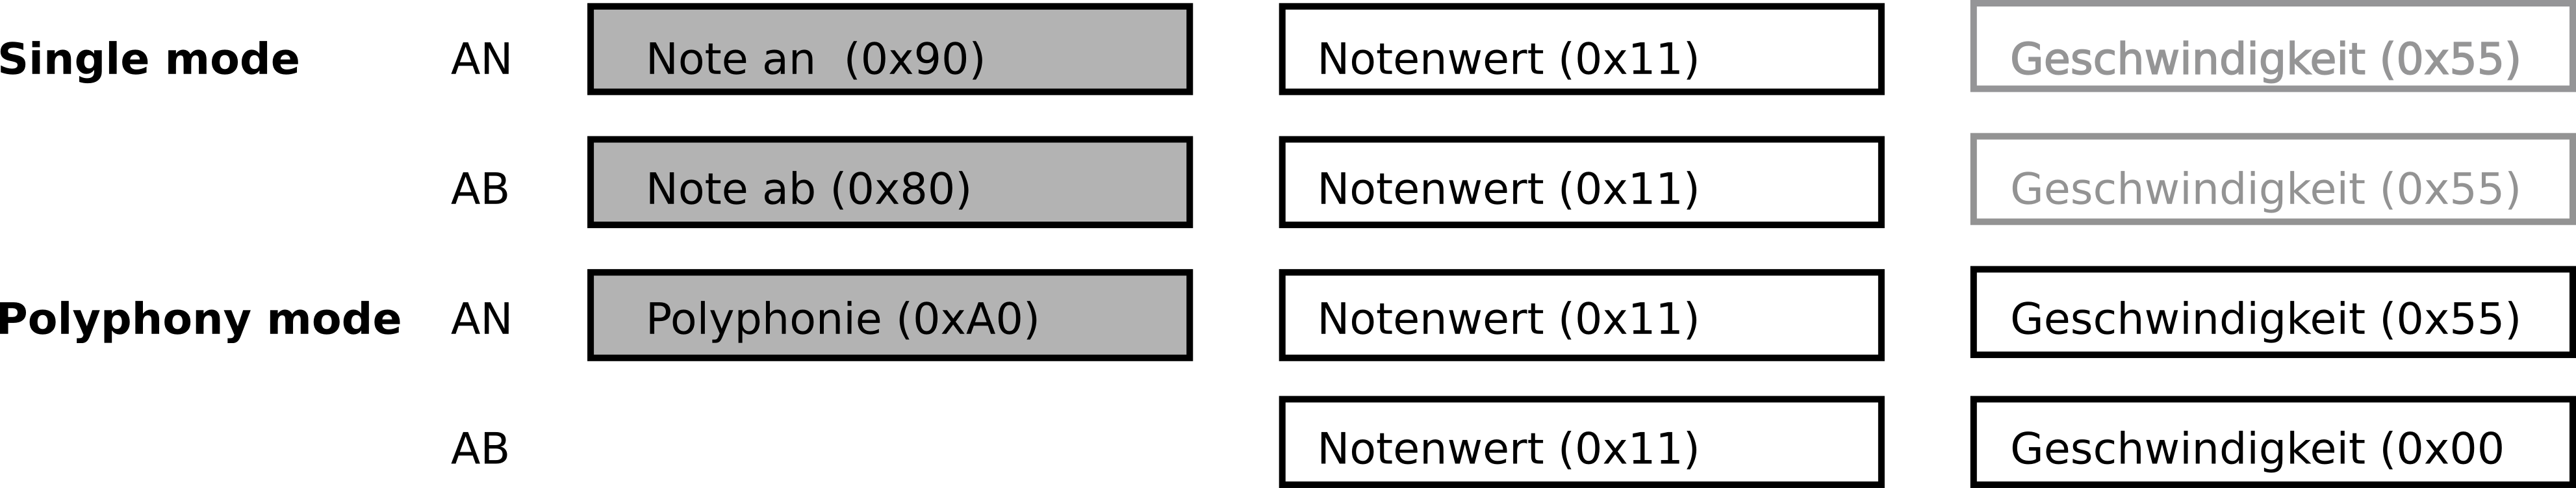
\includegraphics[width=1\textwidth]{images/midi_interface/MIDI_Spezifikation.png}
	\caption{MIDI Spezifikation für Datenstruktur einzelne Note und Polyphonie}
	\label{fig.testbench_single_Mode}
\end{figure}

Unterschiedlich zu behandeln ist die Funktion des Status Bytes. Im Single Mode wird mit dem Status Byte der Zustand an oder ab mitgegeben. Im Polyphony Mode wird nur der Noten-Modus mitgeteilt und das Status Byte hat keine weiteren Funktionalitäten. In der Abbildung wird der Platz von Note an oder ab bezüglich dem Noten-Byte durch graue Markierung veranschaulicht. Die zeitliche Reihenfolge der ist umgekehrt, was in der Token-Verarbeitung berücksichtigt werden muss.

\begin{figure}[H]
	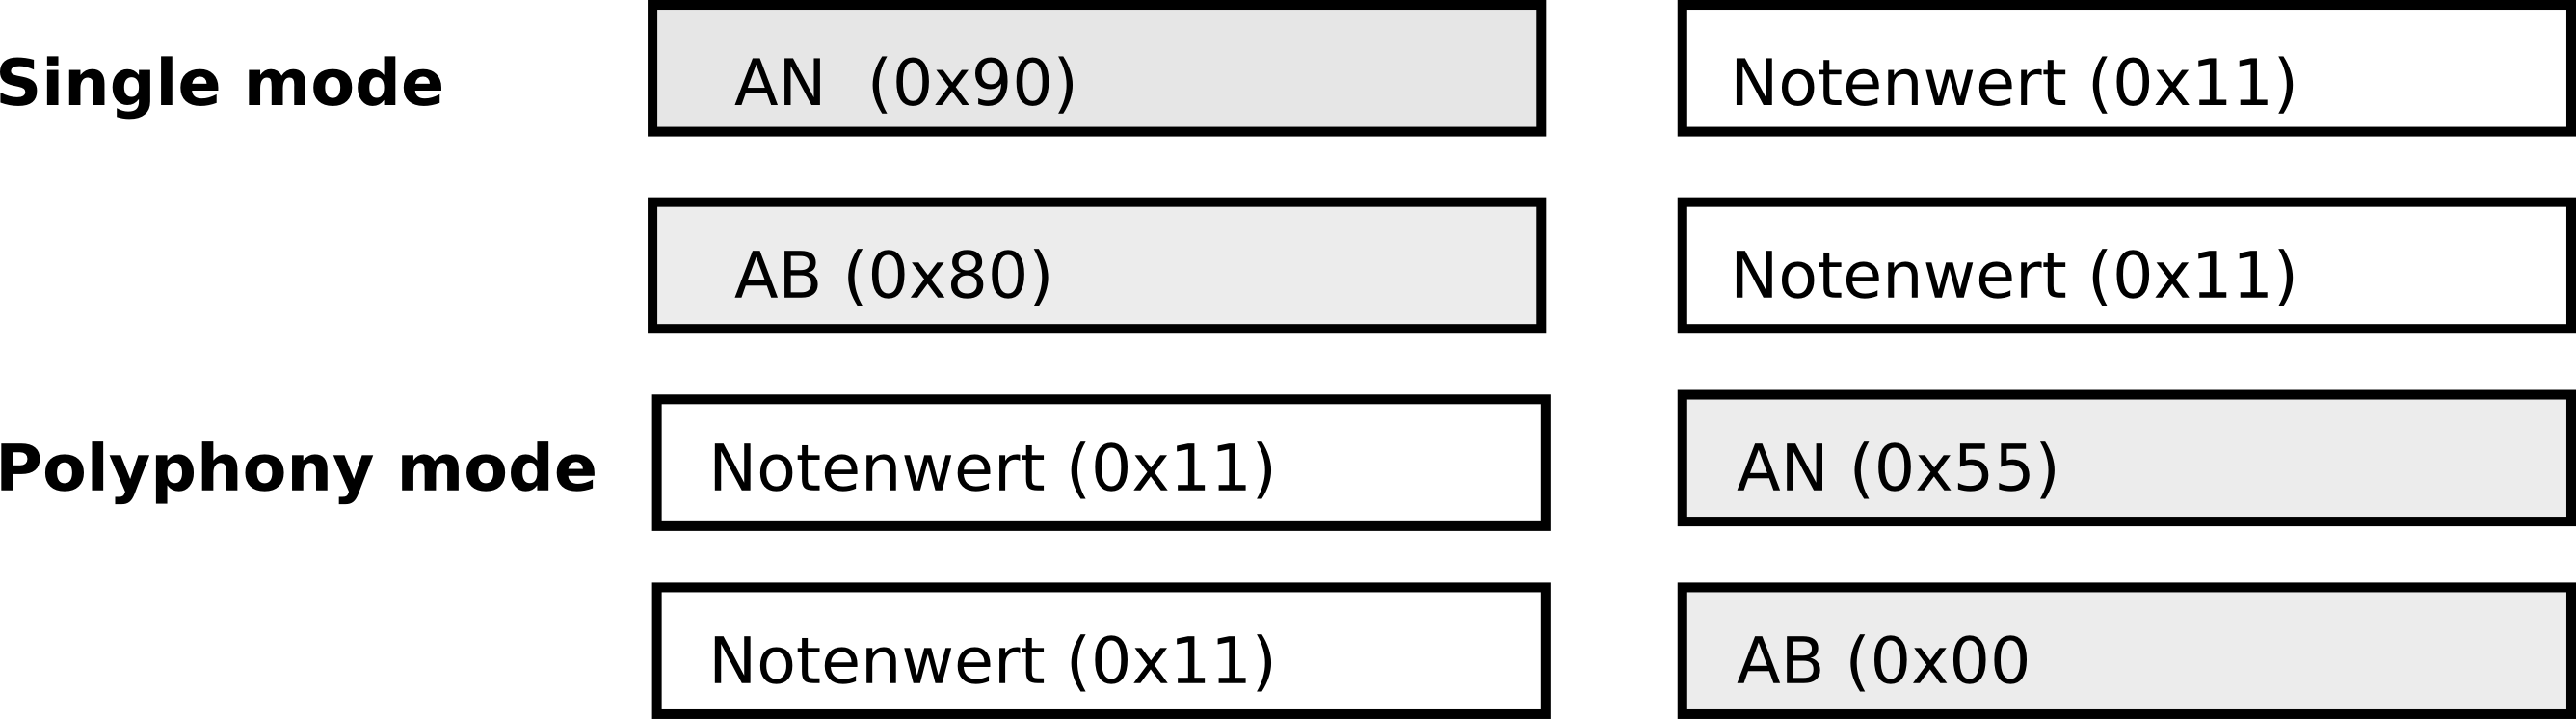
\includegraphics[width=0.7\textwidth]{images/midi_interface/MIDI_Spezifikation_Datenfolge.png}
	\caption{Blockschaltbild Device unter Test}
	\label{fig.testbench_polypphon_mode}
\end{figure}

Wegen der unterschiedlichen Bedeutung der eingegangenen Token, behandelt die FSM die zwei Noten-Modi und deren Noten- und Geschwindigkeitszustände unabhängig voneinander.


\section{MIDI-Steuerung: Blockschaltbild und Schnittstellen}

Analog zum bestehenden Synthesizer-Projekt erhält der VHDL-Block einen englischen Namen: Die MIDI-Steuerung ist als Block mit dem Namen Midi Interface implementiert. Als erstes die Zusammenfassung der internen Blöcke. Die zwei entwickelten Blöcke Midi Control und Polyphony Out sind grau markiert (siehe Abbildung \ref{fig.midi_interface_block} ). Gegeben ist der Block UART top.

\begin{figure}[H]
	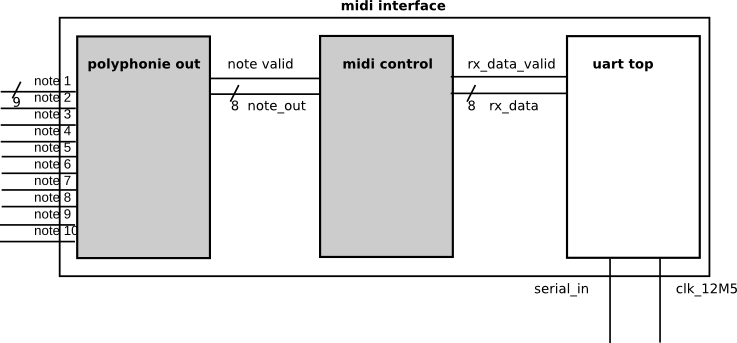
\includegraphics[width=0.7\textwidth]{images/midi_interface/midi_interface_block.png}
	\caption{Blockschaltbild Midi Interface}
	\label{fig.midi_interface_block}
\end{figure}

\textbf{Definition der Schnittstellen}\label{schnittstellen}

UART Top Ausgang

\begin{itemize}
	\item 8-Bit-Signal: Bytweise Dekodierung der Midi Daten 
	\item 1-Bit-Signal: Übermittelt Gültigkeit der Daten
\end{itemize}

Midi Control Ein- und Ausgang

\begin{itemize}
	\item Empfangen von 8-Bit Midi Daten,
    \item Empfangen, ob Daten korrekt sind (1 Bit)
	\item Übermittelt 9-Bit-Notenvektor (Struktur des Vektors in Abb.\ref{fig.Notenvektor})
    \item Übermitteln, ob Daten korrekt (1 Bit)
\end{itemize}

Polyphony Out Ein- und Ausgang

\begin{itemize}
	\item Eingang eines 9-Bit-Notenvektors
    \item Eingang, ob Daten gültig sind
	\item Ausgabe von 10 Notenvektoren zu 9-Bit.
\end{itemize}
\bigskip

Im vorgegebenen Konzept für Polyphony Out (siehe Unterkapitel \ref{konzept_plyphonie}) ist die Schnittstelle zum Polyphony Out-Block als ein 9-Bit-Signal definiert. Das MSB dient als Flag, ob die übermittelte Note an oder ab ist.

\begin{figure}[H]
	
\includegraphics[width=0.2\textwidth]{images/midi_interface/NotenVektor.png}
	\caption{Aufbau Notenvektor}
	\label{fig.Notenvektor}
\end{figure}

Als nächstes wird die MIDI 1.0 Spezifikation, erklärt, nach der Block Midi Control aufgebaut ist. Die Umsetzung des Polyphony Out-Blocks bildet den Abschluss dieses Kapitels.




%------5.3-------------------------------------------------------------
\newpage
\section{Midi Control-Block}\label{sect.midi_umsetzung}

\subsection{Konzept mit Finite State Machine}\label{anforderung_fsm}

Der Controller wird über eine Finite State Machine implementiert. Ausgehend von der Spezifikation \ref{sect.midi_spezification} sind drei Eckpunkte berücksichtigt:

\begin{enumerate}
	\item Unterscheiden von Status Byte und Data Byte
	\item Unterschiedliche Interpretation der Data Bytes abhängig vom Status Byte.
	\item Verwerfen aller falschen Status Byte oder Data Bytes
\end{enumerate}

Vereinfacht verhält sich die FSM wie in Abbildung \ref{fig.midi_fsm_skizze} gezeigt. 

\begin{figure}[H]
	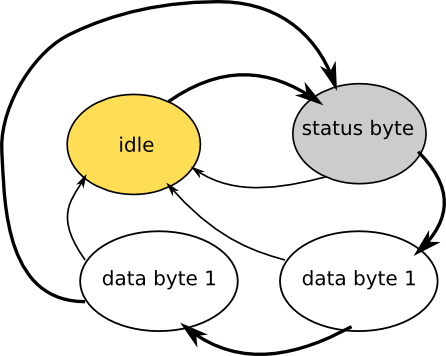
\includegraphics[width=0.3\textwidth]{images/midi_control/fsm_grob_2.png}
	\caption{Skizze der FSM}
	\label{fig.midi_fsm_skizze}
\end{figure}

Startpunkt der Verarbeitung ist das Status Byte (grau hinterlegt). Danach führt die Verarbeitung durch die zwei Data Bytes.\\
In jedem Zustand, werden ungültige Daten verworfen, und führen zurück zu Idle. Die Verarbeitung wird fortgesetzt, wenn das nächste Status Byte folgt.

Nicht angeschrieben sind die Übergangsbedingungen: \lstinline|data_valid = '1'| wechselt zwischen den Zuständen und \lstinline|data_valid = '0'| verbleibt im Zustand. Die breiteren Pfeile heben die fehlerfreie Datenverarbeitung hervor.

\subsection{Implementation der Finite State Machine}

Aufgrund der unterschiedlichen Datenstruktur für den Polyphony Mode und den Single Mode besitzen beide Noten-Modi ihre eigenen Zustände (siehe Abbildung \ref{fig.midi_fsm_detail}).

Die implementierten Zustände sind

\begin{itemize}
	\item \lstinline|idle|: Alle nicht näher spezifizierten Vorfälle verwerfen
	\item \lstinline|single|: Eintreten in  Single Mode durch Status Bytes \lstinline|0x80| oder \lstinline|0x90|
	\item \lstinline|note_s|: Erstes Data Byte im  Single Mode
	\item \lstinline|velocity_s|: Zweites Data Byte im Single Mode
	\item \lstinline|polyphonie|: Eintreten in polyphony mode durch status byte 0xA0
	\item \lstinline|note_v|: Erstes Data Byte im  Polyphony Mode
	\item \lstinline|velocity_v|: Zweites Data Byte im  Polyphony Mode
\end{itemize}
\bigskip

Abbildung \ref{fig.midi_fsm_detail} definiert die Übergangsbedingungen. Drei generelle Verhaltensweisen sind vereinfacht angegeben:

\begin{itemize}
	\item \lstinline|data_valid = '0'|\\
        Im aktuellen Zustand bleiben.\\
        Dargestellt mit Pfeil an Ort
	\item \lstinline|data_valid = '1'|\\
        Grundbedingung für Zustandswechsel\\
        Gilt implizit zu jedem Pfeil und dessen Bedingung dazu
	\item \lstinline|data(7) = '1' and (data(7 downto 5) /= "100" or data(7 downto 4)/= '1010')| \\
        Status Bytes, die nicht Polyphony oder Single Mode bedeuten, verworfen\\
        Dargestellt durch Pfeil oben rechts zu Idle. Gilt für jeden Zustand
\end{itemize}
\bigskip

Die Übergangsbedingungen detektieren die Binärstruktur der MIDI-Daten, die im Unterkapitel \ref{midi_binaer} aufgelistet ist.

\begin{figure}[H]
	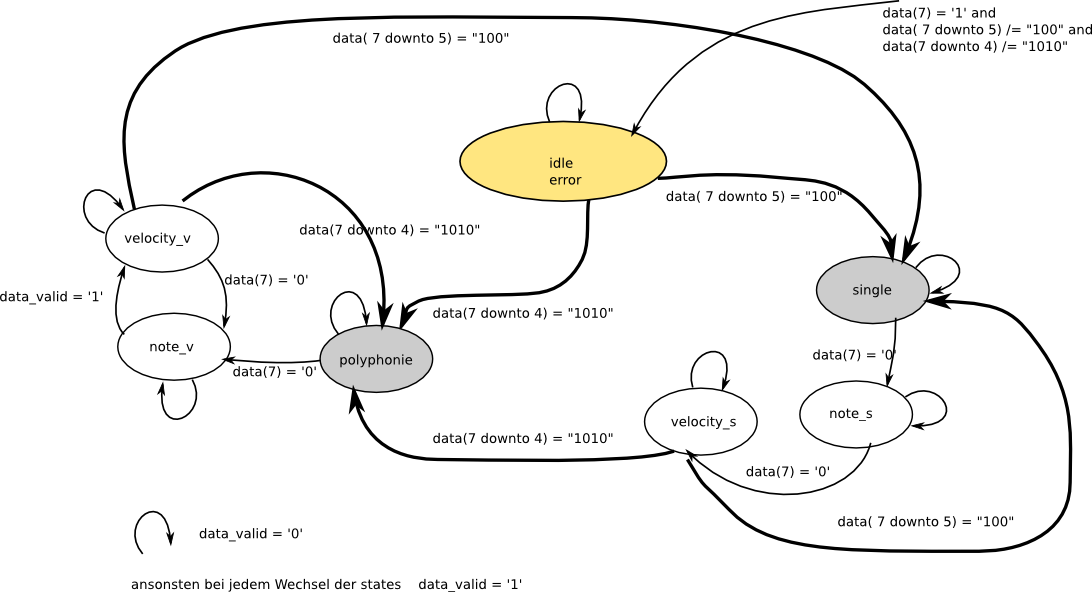
\includegraphics[width=1\textwidth]{images/midi_control/fsm_detailliert.png}
	\caption{Übergänge der FSM}
	\label{fig.midi_fsm_detail}
\end{figure}

Alle drei Anforderungen \ref{anforderung_fsm}, die sich aus der MIDI-Spezifkation ergeben, sind implementiert:

\begin{enumerate}
\item Vor jedem Data Byte muss ein Status Byte eingegangen sein. Die Finite State Machine fragt im Idle Zustand nur nach den Status Bytes. Nach dem Status Byte erwartet die Finite State Machine Data Bytes. 
\item Die unterschiedliche Datenstruktur der zwei Noten-Modi ist Mode-spezifisch implementiert:\\
Im Single Mode wird das vierte Bit des Status Bytes zum Setzen von an und ab verwendet.\\
Im Polyphony Mode wird das zweite Data Byte, die Geschwindigkeit zum Setzen der Note auf an oder ab verwendet.\\
Geschwindigkeit = NULL ist als Note aus implementiert.
\item Ungültige Bytes sind verworfen, und die FSM kehrt in den Idle-Zustand zurück.
\end{enumerate}

%------5.4------------------------------------------------------------
\newpage
\section{Resultat}\label{sect.midi_resultat}

\subsection{Implementierte Finite State Machine}

Abbildung \ref{fig.midi_fsm_quartus_} zeigt die in Quartus generierte FSM des Blocks Midi Control.

\begin{figure}[H]
	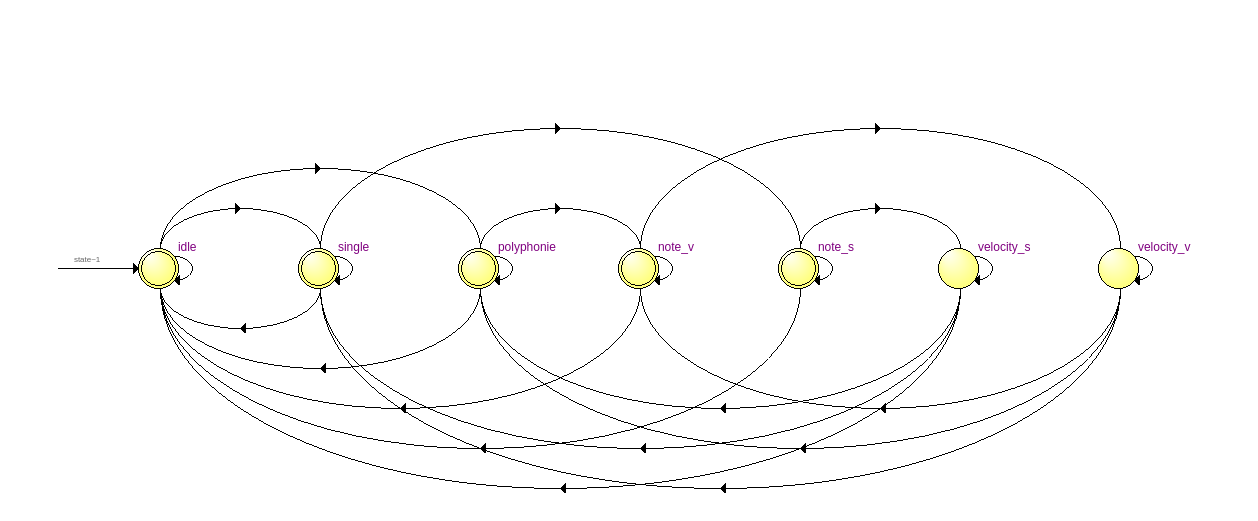
\includegraphics[width=1\textwidth]{images/midi_control/fsm_midicontrol.png}
	\caption{Implementierte FSM im Block Midi Control}
	\label{fig.midi_fsm_quartus_}
\end{figure}

\subsection{Simulation Single Mode}

Der Aufbau der Test Bench und dadurch der Simulation wie auch der Input-Daten ist  in Kapitel \ref{chap.testen} eingehend beschrieben. Hier steht exemplarisch \textit{eine} Auswertung für den Single Mode und im nächsten Unterkapitel für den Polyphony Mode, damit das korrekte Funktionieren der Implementation dokumentiert ist.
 
\textbf{Input Daten} (Zeile 3, siehe Anhang \ref{chap.anhang_midi_input})

{
\renewcommand{\arraystretch}{1.0} % avoid the extra space between the rows
\begin{tabular*}{\textwidth}{@{}@{\extracolsep{\fill}}*{10}{l}@{}} % @{} removes the left and right margin around the table
singl & 55 & 90 & 27 & 80 & 27 & 90 & 02 & 00 & 00
\end{tabular*}
}

\textbf{Beschreibung der Befehle}

\begin{itemize}
\item 55 als Dummy-Velocity für alle Noten
\item Note an
\item Notenwert 27
\item Note ab
\item Notenwert 27
\item Note an
\item Notenwert 02
\item Dummy werte
\end{itemize}

\textbf{Erwartetes Resultat}

Der Kontroller erkennt die Note 27, schaltet diese an und gibt am Ausgang den Vektor \lstinline|"Note-27-AN"| aus. Dieselbe Note wird nochmals detektiert, diesmal als ab und der Vektor am Ausgang zeigt \lstinline|"Note-27-AB"| an. Die nächste Note hat den Wert 2 und wird auf AN gesetzt. Der Ausgang gibt \lstinline|"Note-2-AN"| aus.

\newpage

\begin{figure}[H]
	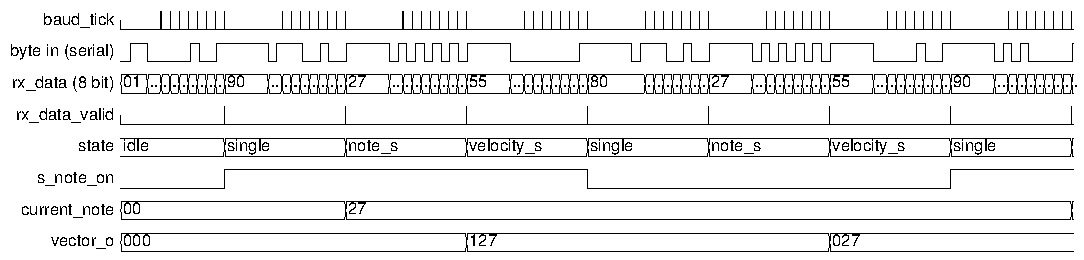
\includegraphics[width=1\textwidth]{images/midi_control/wave_single.png}
	\caption{FSM für Single Mode}
	\label{fig.midicontrol_singlet}
\end{figure}

\begin{itemize}
	\item Das Signal \lstinline|rx_data| detektiert die Befehle \lstinline|(0x90)| und \lstinline|(0x80)|.
	\item Der Controller interpretiert Single Modus. 
	\item Die Zustandsabfolge ist korrekt: \lstinline|single, note_s, velocity_s|.
	\item Die Zustände werden bei \lstinline|rx_data_valid = '1'| geändert.
\end{itemize}

Die Simulation zeigt, dass die Notenwerte korrekt gespeichert sind und dass das An- und Abstellen der Noten funktioniert. Am Ausgang erscheint der zusammengesetzter Vektor aus den 8 Notenbits und einem vorangestellten Bit, das detektiert, ob die aktuelle Note an oder ab ist. 

\subsection{Simulation Polyphony Mode}

\textbf{Input Daten} (Zeile 9, siehe Anhang \ref{chap.anhang_midi_input})

{
\renewcommand{\arraystretch}{1.0}
\begin{tabular*}{\textwidth}{@{}@{\extracolsep{\fill}}*{10}{l}@{}}
polyp & 02 & 55 & 03 & 00 & 20 & 00 & 40 & 55 & 00
\end{tabular*}
}

\textbf{Beschreibung der Befehle}

\begin{itemize}
\item Notenwert 02
\item Note an
\item Notenwert 03
\item Note ab
\item Notenwert 02
\item Note ab
\item Notenwert 4
\item Note an
\end{itemize}

\textbf{Erwartetes Resultat}

Der Kontroller erkennt die Note 02, schaltet diese an und gibt am Ausgang den Vektor \lstinline|"Note-02-AN"| aus. Die Note 03 wird detektiert, auf ab gesetzt und der Vektor am Ausgang zeigt \lstinline|"Note-03-AB"|. Die nächste Note hat den Wert 2 und wird auf ab gesetzt. Der Ausgang gibt \lstinline|"Note-2-Ab"| aus. Als letztes folgt die Note 40, die angestellt wird.

\begin{figure}[H]
	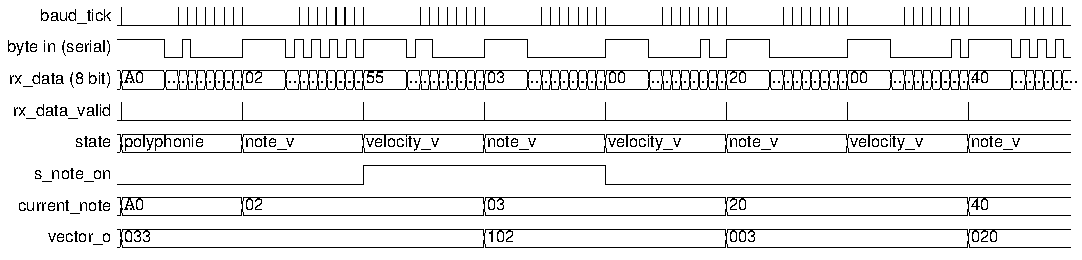
\includegraphics[width=1\textwidth]{images/midi_control/wave_polyphonie.png}
	\caption{FSM im Polyphony Mode}
	\label{fig.midicontrol_polyphonie}
\end{figure}

\begin{itemize}
	\item Das Signal \lstinline|rx_data| detektiert den Befehle (0xA0).
	\item Der Controller interpretiert Polyphony Mode. 
	\item Die Zustandsabfolge ist korrekt: \lstinline|polyphonie, note_v, velocity_v|.
	\item Der Controller wartet mit dem Setzen der Note am Ausgang, bis klar ist, ob die Note an oder ab ist.\\
	Keine kurzfristig falschen Noten am Ausgang, die ab sind.
	\item Zustände werden bei \lstinline|rx_data_valid = '1'| die Zustände geändert.
	\item Noten können beliebig an- und abgestellt werden
\end{itemize}

\section{Polyphony Out-Block}\label{sect.polyphonie_umsetzung}
 
\subsection{Funktionsbeschreibung}

Der Polyphone Out-Block speichert die empfangenen Signale in 10 Registern. Bei jeder neuen Note wird geprüft, ob der Wert im Register besteht und ob das ON/OFF-Bit der gespeicherten neu gesetzt werden muss. Der Block gibt 10 Noten parallel aus.

\begin{figure}[H]
	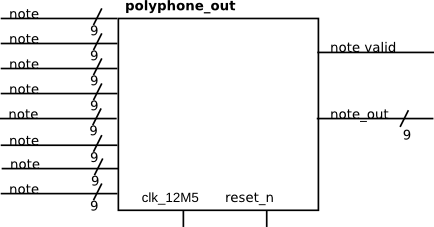
\includegraphics[width=0.5\textwidth]{images/midi_interface/polyphonie_blockschaltbild.png}
	\caption{Polyphone Out-Block}
	\label{fig.polyphnie_out_block}
\end{figure}

\subsection{Konzept}\label{konzept_plyphonie}

Der empfangene Notenwert wird mit den gespeicherten Notenwerten verglichen. Ist eine Note vorhanden, wird das ON-OFF-Bit geprüft und aktualisiert. Keine Note darf zweimal gespeichert sein. Sind alle 10 Registerplätze besetzt, wird die neue Note in ein Register mit abgeschaltetem ON-OFF-Bit gesetzt.

\begin{figure}[H]
	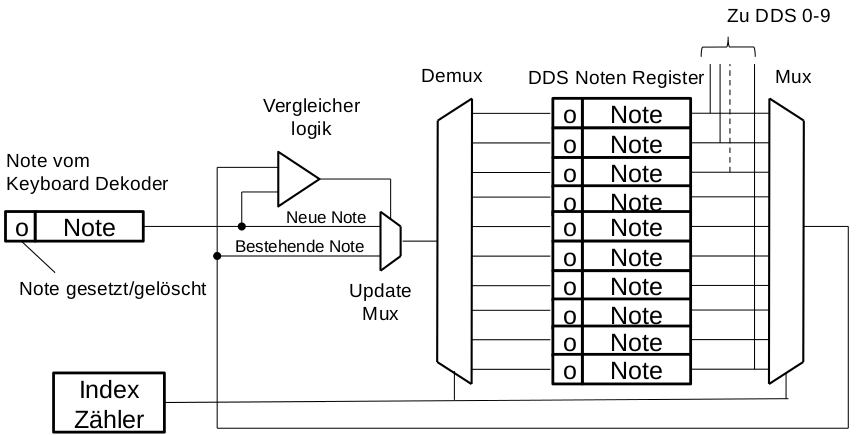
\includegraphics[width=0.7\textwidth]{images/midi_interface/Konzept_Hans_polyphonie.png}
	\caption{Konzept Polyphonie Block \citep{konzept_poly} }
	\label{fig.polyphnie_konzept}
\end{figure}

\subsection{Implementation}

Der Ablauf des Speicher-Vorgangs der neuen Note ist aus der Abbildung \ref{fig.polyphnie_ablauf} ersichtlich.

\begin{figure}[H]
	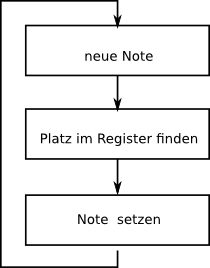
\includegraphics[width=0.2\textwidth]{images/midi_interface/polyphnie_ablauf.png}
	\caption{Ablauf Note speichern }
	\label{fig.polyphnie_ablauf}
\end{figure}

Umgesetzt wird das Suchen eines Speicherplatzes innerhalb der 10 Registern mit einer Input-Logik, die mit folgenden 3 Vergleichen arbeitet:

\begin{enumerate}
	\item Liegt der Notenwert in einem Register ? 
	\item Ist ein Register unbenutzt ?
	\item Welches Register hat einen abgeschalteten Notenwert ?
\end{enumerate}

Sobald eine Frage mit Ja beantwortet wird, wird der Registerindex gespeichert und als Output des Logik-Prozesses zur Verarbeitung weiter gegeben.

Durch den übermittelten Index-Wert weiss der Speicher-Prozess, in welches Register die neue Note gespeichert werden soll.\\
Die Werte aller 10 Register werden am Ausgang parallel ausgegeben.

\section{Resultat}\label{test_polypohnie}

Die Ziele sind:

\begin{itemize}
    \item dass jeder Notenwert in ein anderes Register gespeichert wird und kein Notenwert zweimal abgelegt wird.
    \item An und Ab müssen in dasselbe Register gespeichert werden.
    \item Dieses Konzept ist unabdingbar für den Polyphony Mode und stört die Notenausgabe im Single Mode nicht. 
\end{itemize}


\subsection{Simulation parallel Noten ausgeben}

\textbf{Input Daten} (Zeile 3, 5, 7 und 9 siehe Anhang \ref{chap.anhang_midi_input})

{
\renewcommand{\arraystretch}{1.0}
\begin{tabular*}{\textwidth}{@{}@{\extracolsep{\fill}}*{10}{l}@{}}
singl & 55 & 90 & 27 & 80 & 27 & 90 & 05 & 00 & 00\\
singl & 55 & 90 & 73 & 80 & 73 & 90 & 16 & 00 & 00\\
polyp & 71 & 55 & 02 & 55 & 33 & 55 & 08 & 00 & 00\\
polyp & 20 & 55 & 03 & 00 & 20 & 00 & 40 & 55 & 00
\end{tabular*}
}

\textbf{Beschreibung der Befehle}

\begin{itemize}
\item Dummywert Velocity 0x55
\item Note an 
\item Notenwert 27
\item Note ab 
\item Notenwert 27
\item Note an
\item Notenwert 05
\end{itemize}

\begin{itemize}
\item Dummywert Velocity 0x55
\item Note an
\item Notenwert 73
\item Note ab
\item Notenwert 73
\item Note an
\item Notenwert 16
\end{itemize}

\begin{itemize}
\item Notenwert 71
\item Note an
\item Notenwert 02
\item Note an
\item Notenwert 33
\item Note an
\item Notenwert 08
\item Note ab
\end{itemize}

\begin{itemize}
\item Notenwert 20
\item Note an
\item Notenwert 03
\item Note ab
\item Notenwert 20
\item Note ab
\item Notenwert 40
\item Note an
\end{itemize}

\textbf{Erwartetes Resultat}

\begin{itemize}
\item Note 27 wird angestellt (Vektor ist 127), Note 27 wird abgestellt (Vektor ist 027). An und Abstellen sind in demselben Register abgelegt.
\item Note 05 wird angestellt und in neuem Register abgelegt, da dieses Register unbenutzt ist.
\item Note 73 wird angestellt und nachher abgestellt. Beides in neuem Register.
\item Note 16 wird angestellt und in neues Register gelegt.
\item Note 71 wird angestellt und in neues Register gelegt.
\item Note 02 wird angestellt und in neues Register gelegt.
\item Note 33 wird angestellt und in neues Register gelegt.
\item Note 08 wird abgestellt. (Neues Register stört nicht).
\item Note 20 wird angestellt und in neues Register gelegt.
\item Note 03 wird abgestellt. (Neues Register stört nicht).
\item Note 20 wird abgestellt. Muss im 20-Notenregister sein.
\item Note 40 wird angestellt und in neues Register gelegt.
\end{itemize}

\begin{figure}[H]
	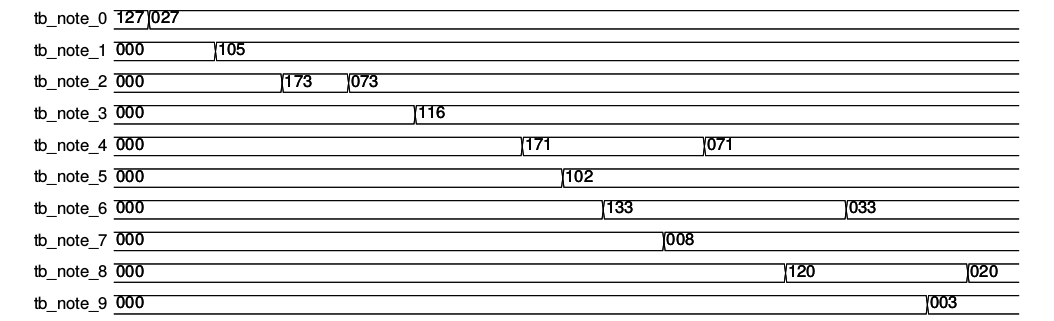
\includegraphics[width=0.8\textwidth]{images/midi_interface/tb_polyphonie.png}
	\caption{Simulation des Blocks Polyphonie Out }
	\label{fig.polyphnie_simulation}
\end{figure}

Die Simulation verhält sich exakt nach Spezifikation.
